\section{Universality}\label{sec:universality}

The first step in Turing's proof is to define the computing model now known as a Turing Machine that we introduced in Chapter~\ref{ch:machines}.  He argued that this simple model corresponds to our intuition about what can be done using systematic computation.  Recall this was 1936, so the model for systematic computation was not what a mechanical computer can do, but what a human computer can do.  Turing argued that his model corresponded to what a human computer could do by following a systematic procedure: the infinite tape was as powerful as a two-dimensional sheet of paper, the set of symbols must be finite otherwise it would not be possible to correctly distinguish all symbols, and the number of machine states must be finite because there is a limited amount a human can remember.  

Next, Turing argued that it is possible to enumerate all Turing Machines.  One way to see this is to devise a notation for writing down any Turing Machine.  A Turing Machine is completely described by its alphabet, states and transition rules.  So, we could write down any Turing Machine by numbering each state and listing each transition rule as a tuple of the current state, alphabet symbol, next state, output symbol, and tape direction.  We can map each state and alphabet symbol to a number, and use this encoding to write down a unique number for every possible Turing Machine.  Hence, we can enumerate all possible Turing Machines by just enumerating the positive integers.  Most positive integers do not correspond to a valid Turing Machine, but if we go through all the numbers we will eventually reach every possible Turing Machine.  

This is already a strong step towards proving that some problems cannot be solved by any algorithm.  The number of Turing Machines is less than the number of real numbers.  Both numbers are infinite, so what does it mean to say there are more real numbers than integers?  This question was resolved by Georg Cantor.  His proof used a technique known as \definition{diagonalization}.  Suppose the real numbers are enumerable.  This means we could list all the real numbers in order, so we could assign a unique integer to each number.  For example, considering just the real numbers between 0 and 1, our enumeration might be:

\begin{tabular}[c]{rl}
1     & $.00000000000000\ldots$ \\
2     & $.25000000000000\ldots$ \\
3     & $.33333333333333\ldots$ \\
4     & $.66666666666666\ldots$ \\
$\cdots$ & $\cdots$ \\
57236 & $.141592653589793\ldots$\\
$\cdots$ & $\cdots$ \\
\end{tabular}

Cantor proved by contradiction that there is no way to enumerate all the real numbers.  The trick is to produce a new real number that is not part of the enumeration.  We can do this by constructing a number whose first digit is different from the first digit of the first number, whose second digit is different from the second digit of the second number, etc.  For the example enumeration above, we might choose $.1468\ldots$.  

The $k^{th}$ digit of the constructed number is different from the $k^{th}$ digit of the number $k$ in the enumeration.  Since the constructed number differs in at least one digit from every enumerated number, it does not match any of the enumerated numbers exactly.  Thus, there is a real number that is not included in the enumeration list, and it is impossible to enumerate all the real numbers.  This suggests that there are real numbers that cannot be produced by any Turing Machine: there are fewer Turing Machines than there are real numbers, so there must be some real numbers that cannot be produced by any Turing Machine.

The next step is to define a \definition{Universal Turing Machine} as depicted in Figure~\ref{fig:universalmachine}.

\begin{figure}[bthp]
\begin{center}
{\scalebox{1.0}{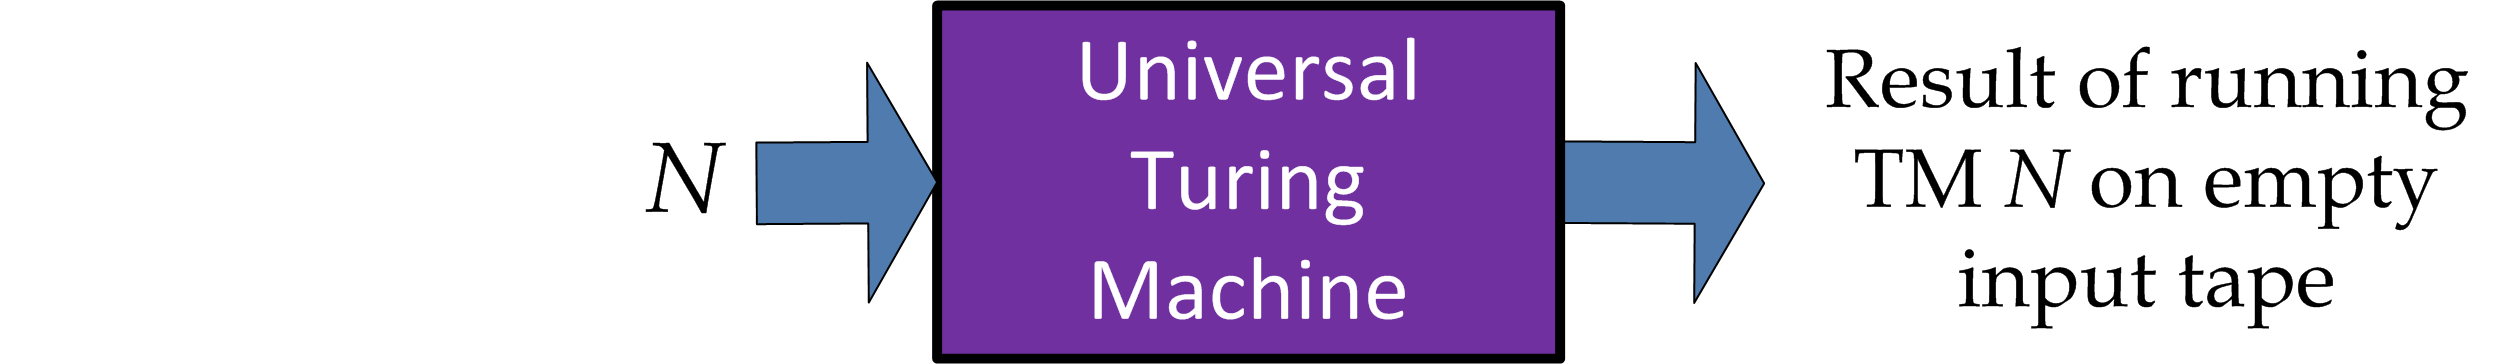
\includegraphics{figures/universal-machine.png}}}
\caption{Universal Turing Machine.}\label{fig:universalmachine}
\end{center}
\end{figure}

A Universal Turing Machine is a machine that takes as input a number that identifies a Turing Machine and a description of an input and simulates the specified Turing Machine on the given input.  The universal machine can simulate any Turing Machine on any input.  In his proof, Turing describes the transition rules for a universal machine.  A universal machine simulates the Turing Machine encoded by the input number.  One can imagine doing this by using the tape to keep track of the state of the simulated machine.  For each step, the universal machine needs to search the description of the input machine to find the appropriate rule.  This is the rule for the current state of the simulated machine on the current input symbol of the simulated machine.  The universal machine keeps track of the machine and tape state of the simulated machine, and simulates each step.  Thus, there is a single Turing Machine that can simulate every Turing Machine.

Using the universal machine and a diagonalization argument similar to the one above for the real numbers, Turing was able to reach a similar contradiction for a problem analogous to the Halting Problem described above for Scheme expressions but for Turing Machines instead.

Since a Universal Turing Machine can simulate every Turing Machine, and a Turing Machine can perform any computation according to our intuitive notion of computation, this means a Universal Turing Machine can perform all computations.  If we can simulate a Universal Turing Machine in a programming language, that language is a \definition{universal programming language}.  There is some program that can be written in that language to perform every possible computation.  It is sufficient to show that it can simulate a Universal Turing Machine, since a Universal Turing Machine can perform every possible computation.  To simulate a Universal Turing Machine, we need some way to keep track of the state of the tape (for example, a List in Scheme would be adequate), a way to keep track of the internal machine state (a Number in Scheme can do this), and a way to execute the transition rules (we could define a Scheme procedure that does this, using an if-expression to make the decision about which transition rule to follow).  Thus, Scheme is a universal programming language: one can write a Scheme program to simulate a Universal Turing Machine, and thus, perform any mechanical computation.
